% ---------------------------------------- %
%       Preamble / options / packages      %
% ---------------------------------------- %
\documentclass[10pt,a4paper]{article}
\author{
    ---------------  Add Authors List here  ---------------
}
\usepackage{graphicx}
\usepackage{biblatex} 
\usepackage{threeparttable}
\usepackage{tabularx}
\usepackage[hidelinks]{hyperref}
\usepackage[left=2.5cm,right=2.5cm,top=3cm,bottom=3cm]{geometry}
\usepackage{amsmath}
\usepackage{bbm}
\usepackage{booktabs}  % for compatibility with table generated by pandas.to_latex()

\usepackage{tikz, lmodern}
\usetikzlibrary{calc,tikzmark}

\renewcommand{\thefigure}{S\arabic{figure}}
\renewcommand{\thetable}{S\arabic{table}}

% code below is to add a new sectioning level (e.g. 2.1.3.4)
% this new level will be requested using the \paragraph{} command
\usepackage{titlesec}
\setcounter{secnumdepth}{4}
\titleformat{\paragraph}
{\normalfont\normalsize\bfseries}{\theparagraph}{1em}{}
\titlespacing*{\paragraph}
{0pt}{3.25ex plus 1ex minus .2ex}{1.5ex plus .2ex}
 
\setlength{\abovecaptionskip}{-8pt}  % reduce the margin between figures and captions
% TeX code to create a custom command called \code to allow for the inclusion of inline code
\usepackage{xcolor}
\definecolor{light-gray}{gray}{0.9}  % Define the background colour
\newcommand{\code}[1]{\colorbox{light-gray}{\texttt{#1}}}  % Manual creation of an inline code command

\bibliography{./school_closure_library}

\title{
    Estimating the impact of school closures on COVID-19 disease burden\\
    \Large Supplementary Appendix
}

\date{\vspace{-5ex}} % This removes the date from the title page


% ---------------------------------------- %
%       Document really starting here      %
% ---------------------------------------- %
\begin{document}
\maketitle
\tableofcontents
\newpage
% This file describes the general structure of some of our tb_dynamics models.

\section{Model Structure}

\subsection{General features}

We use a deterministic compartmental model including six types of compartments that represent 
different states of infection and disease. The model uses the same conceptual approach and similar 
assumptions to previously published models \cite{trauer-2017, ragonnet-2019, ragonnet-2021, ragonnet-2022}. 
Here we describe the model structure without treatment compartment and related factors. 
\newline
A susceptible compartment (S) is used to represent individuals who have 
never been infected with \emph{Mycobacterium tuberculosis (M.tb)}. Latent TB infection (LTBI) is modelled 
using two successive compartments: early latent (E) and late latent (L) to capture the declining risk of 
disease progression over time from infection \cite{ragonnet-2017}. The active disease compartment (I) represents 
individuals who have progressed to the active stage of TB disease. Diseased individuals who recover 
through self-cure progress directly to the recovered compartment (R).
\newline
Non-TB-related mortality is modelled by applying death rates to all model compartments. In addition, 
disease-specific mortality is implemented by applying increased mortality rates to the active disease 
compartments (I).
\newline
Reinfection occurs in the model in two different ways. First, latently infected individuals may be 
reinfected, with this process modelled using a flow from the late latent (L) to the early latent 
compartment (E). Second, individuals who have recovered from TB disease may be reinfected and 
return to the early latent compartment. The structure of our model allows for differential risk of 
infection for the currently and previously infected individuals, compared to the infection-naive 
individuals.
\begin{figure}[!htp]
    \vspace*{-1cm}
    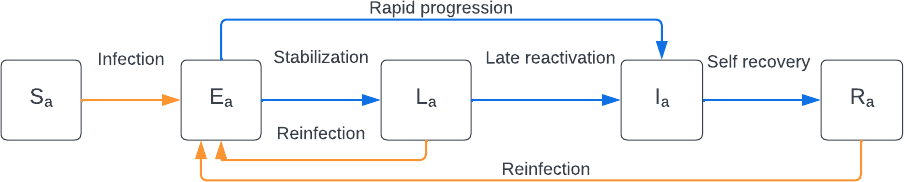
\includegraphics[width=\textwidth,height=\textheight,keepaspectratio]{images/model.png}
    \caption{Illustration of the model structure. 
    Boxes represent the different compartments types: susceptible (S), early latent (E), late latent (L), infectious (I), and recovered (R).
    The subscript indicates that compartments are stratified by age (a).}
    \label{fig:model}
\end{figure}

\subsection{Stratification by age}
The model is stratified using five categories: 0-4, 5-14, 15-34, 35-49 and 50+ years old. We assume 
heterogeneous mixing by age using an age-specific contact rate matrix. Since no local estimates of 
contact patterns by age were available for the Marshall Islands, we used a contact survey conducted in 
the Fijian population and adjusted the estimates to account for age distribution differences between
the two countries.


\section{Software and code used to conduct the analyses}

\subsection{Code}
The Python code and data used to perform the analyses is fully available on Github at the following link:
\href{https://github.com/monash-emu/AuTuMN}{https://github.com/monash-emu/AuTuMN}. In particular, \textcolor{red}{LIST LINKS TO SOME SUB-MODULES HERE}.


\subsection{Software implementation}

We used the \textit{summer} Python package (v 1.2.5) to implement the model \cite{summer2024}. This is a domain-specific library for 
compartmental epidemiological modelling enabling highly expressive programming and accelerated computation through Google’s \textit{jax} library

\subsubsection{Application Programming Interface (API)}
The model specification was done via a simple yet expressive Python API, 
while the numerical implementation was autogenerated by the \textit{summer} package at runtime. 
This specification is composable via stratification classes and other reusable components, 
such that the complexity of the software is kept to a minimum, reducing cognitive overhead and greatly reducing the possibility for error.

\subsubsection{Optimising compiler}
The \textit{summer} package uses the jax library as its computational backend, meaning that while the specification of models is done largely in Python, 
the model execution itself is transformed via an optimising compiler into fast native code.
This brings the model runtime from several seconds (for a naive implementation) to under 50ms per iteration, which was necessary to perform the computationally-intensive
calibration tasks described in Section \ref{calibration}.






\section{Model calibration and uncertainty propagation}
\label{calibration}
\textcolor{red}{REVISE THE SECTION BELOW WHEN FINALISED}
The model was calibrated using a Bayesian approach. In particular, we used the adaptive 
Metropolis algorithm introduced by Haario \textit{et al.} to sample parameters from their 
posterior distributions \cite{haario-2001}. For each country, we ran 8 independent Metropolis 
chains initialised using Latin Hypercube Sampling based on the parameter priors. 
We ran simulations for X hours per chain in order to achieve at least 50,000 iterations per 
chain. We discarded the first 25,000 iterations of each chain as burn-in and combined the 
samples of the 8 chains to project epidemic trajectories over time. 
For each modelled country, the epidemic projections presented in our analysis are associated with 1000 parameter sets 
randomly sampled from the posterior distributions obtained from MCMC sampling. 
The definitions of the prior distributions and the likelihood are detailed in the following sections.

\subsection{Parameters varied during calibration}

The parameters varied during calibration along with their associated prior distributions 
are listed in Table (\textcolor{red}{add ref to table here}) and indicated with the superscript \textsuperscript{c}.
We used uniform prior distributions for all calibrated parameters. The primary parameters varied during calibration are 
the unadjusted risk of transmission per contact ($\beta$), the IFR multiplier ($m_C$), the infection seeding times of 
each strain and the proportion of students on-site during ``Partially open'' periods. Note that the values of the random 
process $W_t$ described in Section \ref{random_process} are also treated like calibrated parameters by the MCMC. 
They are associated with an improper uniform prior distribution, whereas the auto-regressive component described in 
Equation \ref{eq:random_process} is incorporated in the posterior likelihood computation (Section \ref{likelihood}).

\subsection{Calibration targets}
\label{targets}
For each country model calibration is achieved by targeting two COVID-19 burden indicators: the 
reported number of COVID-19 deaths over time and country-level seroprevalence estimates. 

We used the daily number of COVID-19 deaths reported by Our World in Data and applied a 7-day moving average to the observed data. 
We used the online platform SeroTracker to extract country-specific seroprevalence estimates.
\textcolor{red}{Use Angus' description here.}

\subsection{Likelihood definition}
\label{likelihood}
Let $d_w$ denote the rounded average daily number of COVID-19 deaths during week $w$, and $\hat{d_w}^\theta$ 
the associated predicted number of deaths according to the model with parameter set $\theta$. 

Let us denote $m$ the sample size associated with the seroprevalence survey selected from SeroTracker (Section \ref{targets}), 
and $k$ the number of seropositive individuals observed in the survey.
Let $\hat{\pi}^\theta$ denote the modelled proportion ever infected by the time the survey was conducted (using midpoint date) 
associated with the parameter set $\theta$. 
The likelihood was defined as follows:

\begin{equation}
    \label{eq:likelihood}
    \mathcal{L}(\theta) := f_{m,\hat{\pi}^\theta}(k) \times \prod_w g_r(d_w | \:\hat{d_w}^\theta) \quad ,
\end{equation}
where $f_{n,p}(.)$ is the probability mass function of a binomial distribution $\mathcal{B}(n,p)$, and 
$g_r(. | \mu)$ is the probability mass function of a negative binomial distribution with mean $\mu$ and 
overdispersion parameter $r$. The parameter $r$ is automatically estimated by the MCMC algorithm.

The likelihood described above represents the goodness of fit of a particular model parameterisation with regards to the targeted data. 
This quantity needs to be adjusted for the prior likelihood of the parameter set in order to compute the MCMC acceptance quantity $\mathcal{Q}(\theta)$.
As we used uniform priors for all the parameters, the inclusion of the individual parameters' priors in the acceptance quantity is not necessary. 
Indeed, their respective contributions would cancel out as the same quantity would appear in the numerator and the denominator of the 
MCMC acceptance quantity ratio. However, the auto-regressive relationship described in Equation \ref{eq:random_process}
must be accounted for as part of the combined prior likelihood of a parameter set. This is what prevents unrealistic fluctuations of the random process.
If $W^\theta$ represents the random process associated with the parameter set $\theta$, the overall MCMC acceptance quantity is obtained by:

\begin{equation}
    \label{eq:acc_qtt}
    \begin{split}
    \mathcal{Q}(\theta) & = \mathcal{L}(\theta) \times \prod_{i=1}^{n} z_{W^\theta_{i-1},\sigma}(W^\theta_i) \\
                        & = f_{m,\hat{\pi}^\theta}(k) \times \prod_w g_r(d_w | \:\hat{d_w}^\theta) \times \prod_{i=1}^{n} z_{W^\theta_{i-1},\sigma}(W^\theta_i) \quad ,
    \end{split}
\end{equation}
where $z_{\mu,\sigma}(.)$ represents the probability density function of the normal distribution $\mathcal{N}(\mu, \sigma)$, and $n$ is the number 
of random process updates. The standard deviation $\sigma$ is automatically estimated by the MCMC.

\subsection{Model coding and run time}
\textcolor{red}{NEED TO COMPLETE THIS. Maybe David can help here?}
Can probably find a better title for this section\dots

We used the \textit{summer} Python package (v 1.2.5) to implement the model \cite{summer2024}. This is a domain-specific library for 
compartmental epidemiological modelling enabling highly expressive programming and accelerated computation through Google’s \textit{jax} library

\subsubsection{Application Programming Interface (API)}
The model specification was done via a simple yet expressive Python API, 
while the numerical implementation was autogenerated by the \textit{summer} package at runtime. 
This specification is composable via stratification classes and other reusable components, 
such that the complexity of the software is kept to a minimum, reducing cognitive overhead and greatly reducing the possibility for error.

\subsubsection{Optimising compiler}
The \textit{summer} package uses the jax library as its computational backend, meaning that while the specification of models is done largely in Python, 
the model execution itself is transformed via an optimising compiler into fast native code.
This brings the model runtime from several seconds (for a naive implementation) to under 50ms per iteration, which was necessary to perform the computationally-intensive
calibration tasks described in Section \ref{calibration}.







\newpage
\printbibliography

\end{document}
